\section{Probabilidad}
La probabilidad es la rama de las matemáticas que cuantifica el grado de certeza o posibilidad de
que ocurra un determinado suceso dentro de un experimento aleatorio. En la investigación
estadística, su teoría es fundamental para modelar la incertidumbre, analizar variables complejas y
fundamentar la toma de decisiones a partir de los datos observados de una población. En esta sección
trabajaremos con las siguientes variables:
\Variable{'career\_specialization\_level'} y \Variable{'gender'}.

\subsection{Tabla de datos}
\begin{TablaDatosFlexible}
  {
    L{0.2\linewidth}
    C{0.15\linewidth}
    C{0.15\linewidth}
    C{0.15\linewidth}
    C{0.15\linewidth}}
    {
      \textbf{Género} &
      \textbf{Básica (B)} &
      \textbf{Media (M)} &
      \textbf{Alta (A)} &
      \textbf{Total}
    }

\TablaFilaFlexible{Femenino (F) & 23 & 19 & 16 & 58}
\TablaFilaFlexible{Hombre (H) & 17 & 11 & 25 & 53}
\TablaFilaFlexible{Total & 40 & 30 & 41 & 111}

\end{TablaDatosFlexible}


\subsection{Gráfico: Barras agrupadas}
\begin{figure}[H]
    \centering
    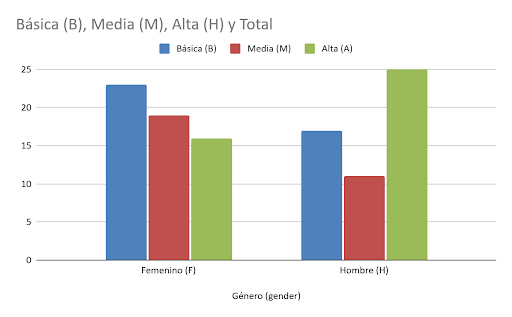
\includegraphics[width=0.7\textwidth]{img/probabilidad.png}
    \caption{Gráfico para las variables \Variable{gender} y \Variable{career\_specialization\_level}.}
    \label{fig:grafico_probabilidad_barras}
\end{figure}


\subsection{Preguntas}

\subsubsection{Pregunta 1: Probabilidad marginal}

¿Cuál es la probabilidad de que una persona seleccionada al azar tenga una especialización alta
(A)?

\paragraph{Respuesta:} 
\[ P(A) = \frac{41}{111} \approx 0.3694 = 36.94\% \]

\paragraph{Interpretación:} Existe una probabilidad del 36,94\% de que cualquier estudiante
seleccionado al azar tenga una especialización alta, independientemente de su género.

% --------------------------------------------------------------------------------------------------

\subsubsection{Pregunta 2: Probabilidad conjunta}

¿Cuál es la probabilidad de elegir al azar a alguien que sea hombre y tenga una especialización
media (M)?

\paragraph{Respuesta:} 
\[ P(H \cap M) = \frac{11}{111} \approx 0.0991 = 9.91\% \]

\paragraph{Interpretación:} Muestra que el 9.91\% del total de los estudiantes de la
muestra son hombres con una especialización media.

% --------------------------------------------------------------------------------------------------

\subsubsection{Pregunta 3: Probabilidad de la unión}

¿Cuál es la probabilidad de elegir a alguien que sea mujer o tenga una especialización básica (B)?

\paragraph{Respuesta:} 
\[ P(F \cup B) = P(F) + P(B) - P(F \cap B) \]
\[ P(F \cup B) = \frac{58}{111} + \frac{40}{111} - \frac{23}{111} = \frac{75}{111} \approx 0.6757 = 67.57\% \]

\paragraph{Interpretación:} Da un 67,57\%. Resta la intersección (las 23 mujeres de nivel básico)
para no duplicar personas en el conteo.

% --------------------------------------------------------------------------------------------------

\subsubsection{Pregunta 4: Probabilidad condicional}

Dado que elegimos a un hombre, ¿cuál es la probabilidad de que tenga una especialización alta (A)?

\paragraph{Respuesta:} 
\[ P(A \mid H) = \frac{25}{53} \approx 0.4717 = 47.17\% \]

\paragraph{Interpretación:} Al cerrarnos solo en los hombres, el porcentaje de alta especialización
sube al 47,17\% (casi la mitad del grupo).

% --------------------------------------------------------------------------------------------------

\subsubsection{Pregunta 5: Prueba de independencia}

¿Son \Variable{gender} y \Variable{career\_specialization\_level} independientes?

\paragraph{Respuesta:} 
\[ P(F \cap A) = \frac{16}{111} \approx 0.1441 = 14.41\% \]
\[ P(F) \cdot P(A) = \frac{58}{111} \cdot \frac{41}{111} \approx 0.5225 \cdot 0.3694 = 0.1929 = 19.29\% \]

\paragraph{Interpretación:} Como la probabilidad real (14,41\%) difiere de la teórica (19,29\%), se
demuestra matemáticamente que el género influye y está asociado a las metas profesionales de los
alumnos.
